% COMSYS Seminar/Preseminar Paper Template
% ----------------------------------------
% Based on the original IEEE template package, includes annotations by COMSYS

\documentclass[conference]{IEEEtran}

%\IEEEoverridecommandlockouts
\usepackage{amsmath,amssymb,amsfonts}
\usepackage{algorithmic}
\usepackage[hidelinks]{hyperref}
\usepackage[capitalize,nameinlink]{cleveref}
\usepackage[sort]{cite}
\usepackage[inline]{enumitem}
\usepackage{balance}
\usepackage{graphicx}
\usepackage{textcomp}



% Prevent subcaption package from overwriting the IEEE template defaults
\makeatletter
\let\SafeCaption\@makecaption
\makeatother
\usepackage{subcaption}
\makeatletter
\let\@makecaption\SafeCaption
\makeatother

\def\BibTeX{{\rm B\kern-.05em{\sc i\kern-.025em b}\kern-.08em
    T\kern-.1667em\lower.7ex\hbox{E}\kern-.125emX}}

\begin{document}

\title{Modern Congestion Control Algorithms}

\author{\IEEEauthorblockN{Yannik Schreiter}
\IEEEauthorblockA{\textit{COMSYS} \\
\textit{RWTH}\\
Aachen, Deutschland \\
Yannik.Schreiter@rwth-aachen.de}
}

\maketitle

\begin{abstract}
Congestion Control Algorithms are critical for regulating data flow and optimizing resource utilization in modern networks. 
This paper provides a comprehensive overview of contemporary Congestion Control Algorithms, tracing the evolution from foundational protocols to highly specialized modern advancements. 
We first establish a theoretical framework by examining traditional loss-based and delay-based algorithms, including TCP Cubic, TCP Vegas, and FAST TCP, while detailing the metrics used to evaluate their performance and fairness.  

The core of this work surveys recent state-of-the-art developments, specifically focusing on BBR and Copa, alongside their respective extensions—AQDC-BBR, BBR-ES, Copa+, and Copa-D—which aim to mitigate issues like "bufferbloat" and RTT unfairness. 
We further explore emerging architectural paradigms such as Performance-oriented Congestion Control (PCC), which utilizes online learning, PowerTCP, which leverages In-band Network Telemetry (INT) for datacenters, and C4, designed for real-time media over unstable wireless links. 
Finally, we provide a comparative analysis of these algorithms based on their design objectives and performance data. 
Our synthesis identifies a trend toward high specialization for distinct environments—such as 4G and 5G mobile networks and datacenters—while highlighting the ongoing challenge of maintaining architectural simplicity and fairness in an increasingly diverse multi-protocol global internet.

\end{abstract}

\begin{IEEEkeywords}
congestion control
\end{IEEEkeywords}

\section{Introduction}

\ac{CCA} are a cornerstone of modern network technology, serving as essential mechanisms to regulate data flow and optimize the utilization of network resources. 
\ac{CCA} is an key topic to the internet as a whole and its being researched since over 40 years so far.
Althought this is a long time, there are still improvements done and research is also actively done.
The importance of \ac{CCA} is that it can be the driving factor to achieve low latency and high thoughtput as well as helping to improve other characteristics of the internet.

This paper provides a comprehensive overview of contemporary \acs{CCA}, examining their operational logic and comparing them through the lens of their design objectives.
To establish a foundational understanding, Section \ref{sec:Background} presents the necessary theoretical background and common performance metrics. 
This section explores established protocols such as TCP Cubic, TCP Vegas, and FAST TCP, while detailing the metrics used to evaluate their efficacy.

In Section \ref{sec:Approach}, we survey recent advancements in the field, specifically focusing on Bottleneck Bandwidth and Round-trip propagation time (BBR) and Copa, alongside both of their extensions. 
We also highlight several other emerging algorithms that represent the current state of the art.
Finally, Section \ref{sec:Evaluation} provides a comparative analysis of these algorithms, evaluating them based on the performance data and architectural goals provided by their respective authors. 
We conclude by situating our findings within the broader academic context, referencing existing literature that offers deeper empirical evaluations of these protocols.
We conclude the paper in Section \ref{sec:Summary} by summarizing our findings and synthesizing the key takeaways from our comparison. 
Furthermore, we provide an outlook in Section \ref{sec:Outlook} on the future of the field, identifying potential trends and remaining challenges in the evolution of congestion control.


\section{Background}

\subsection{Congestion Control general Information}

\subsubsection{Difference between Congestion Control and Congestion Avoidance} <-- Naja, eher unwichtig

\subsubsection{Measuring Indicies}

Jains Index \cite{JainsIndex}

\subsubsection{Types of Congestion Controls}

loss-Based

delay-Based

congestion-Based

\subsubsection{Places of deployment}

Short distance networks

long distance networks

data center

satelite links

small buffer at Bottleneck

large buffer at Bottleneck

\subsection{TCP Vegas}

\cite{TCPVEGAS}

\subsection{TCP Cubic}

\cite{TCPCUBIC}

\subsection{Fast TCP}

\cite{FASTTCP}


\input{Sections/Goal.tex}


\section{Approaches to control congestion}\label{sec:Approach}

Now with the goal set, we can have a closer look on possible approaches that are more new.
These approaches are less than ten years old and represent the best and most known \ac{CCA}s.

\subsection{Bottleneck Bandwidth and Round-Trip propagation Time (BBR)}

BBR was developed by Google researchers to address fundamental inefficiencies in traditional loss-based \acs{CCA}s \cite{BBRORIGINAL}. 
The authors argue that modern hardware advancements have made the long-standing practice of using packet loss as a measure for congestion increasingly problematic. 
Specifically, in environments with large network buffers, loss-based algorithms like CUBIC tend to keep buffers full, leading to "bufferbloat" where delays are measured in seconds rather than milliseconds . 
Conversely, in long-distance networks, packet loss may occur due to link errors rather than actual congestion.
However, loss-based algorithms misinterpret these signals, causing them to reduce throughput unnecessarily \cite{BBRORIGINAL}.

BBR operates through a state machine consisting of a Startup phase and two repeating steady-state phases known as ProbeBW and ProbeRTT\cite{BBREVALUATION}. 
The authors define the optimal operating point as having a delivery rate equal to the bottleneck bandwidth ($BtlBw$) and a total amount of inflight data equal to the pipe's \ac{BDP} \cite{BBRORIGINAL}. 
During the Startup phase, BBR rapidly discovers the bottleneck's limits by increasing its sending rate by a pacing gain of $2/\ln 2 \approx 2.885$ every round trip until the delivery rate plateaus.
While this ensures the bottleneck is discovered in $\log_2 BDP$ rounds, it may temporarily fill the queue with up to $2BDP$ of excess data before transitioning into a Drain phase to empty the buffer \cite{BBRORIGINAL, BBREVALUATION}.

In steady-state operation, the algorithm primarily cycles through the ProbeBW phase to measure and adapt to changes in available bandwidth. 
This phase uses an eight-step cycle where the algorithm typically increases its sending rate by a pacing gain of 1.25 for one \ac{RTT} to probe for additional capacity, then immediately reduces it to a gain of 0.75 for one \ac{RTT} to drain the queue created during the probe \cite{BBREVALUATION}. 
Finally, to refresh the minimum round-trip time estimate, BBR enters the ProbeRTT phase if a lower \ac{RTT} has not been observed for 10 seconds. 
During this phase, the algorithm abruptly limits inflight data to a minimal amount—typically 4 packets—for at least 200 ms to fully drain the bottleneck buffer and measure the true propagation delay of the path \cite{BBRORIGINAL, BBREVALUATION}.

\subsubsection{Active Queue Debt Compensation (AQDC) BBR}

BBR utilizes the ProbeBW phase to estimate available bandwidth by periodically increasing its pacing rate. 
However, this process often injects bursts of traffic that exceed the path's instantaneous capacity, creating temporary queues. 
The authors of \cite{AQDCBBR} identify a critical limitation: these transient queues may not be completely drained during the subsequent ProbeDown phase, leading to a residual queue buildup that accumulates over successive cycles. 
Over time, this results in an upward drift of \ac{RTT} measurements and increased tail latency, which is particularly detrimental to delay-sensitive applications like video streaming.

Furthermore, the authors contend that BBR's ProbeRTT mechanism is rigid and ``blind'' to queue history, as it resets at fixed intervals regardless of the actual backlog. 
To reconcile the conflict between fairness and low latency, AQDC-BBR explicitly models the ``queue debt'' ($B_{total}$) incurred during bandwidth probing. 
This debt is then compensated for by adjusting the target inflight data:

\begin{equation}
    Inflight_{target} = BDP - B_{total}
\end{equation}

By proportionally reducing the inflight data based on the tracked debt, AQDC-BBR drains accumulated queues and restores accurate minRTT tracking without the need for aggressive or heuristic rate cuts.

\subsubsection{BBR-Extended State (BBR-ES)}
BBR exhibits significant \ac{RTT} unfairness when flows with heterogeneous \acs{RTT} share a bottleneck\cite{BBRES}. 
In deep-buffer environments, long-RTT flows tend to dominate bandwidth because they maintain larger inflight data volumes—proportional to their RTT—which allows them to occupy the bottleneck queue more aggressively. 
This leads to a positive feedback loop: higher queue occupancy results in higher delivery rate reports, which further inflates a flow's estimated bandwidth and sending rate. 
While \ac{BBR} ProbeRTT phase is intended to synchronize flows and provide a "fair starting point" by draining the queue, the authors found that it often fails because the algorithm lacks an explicit mechanism to correct accumulated queue imbalances upon exiting this state. 
Consequently, prior imbalances are immediately reintroduced and amplified, a phenomenon the authors describe as the "inaction" of BBR.

To resolve these issues, the authors introduced BBR-ES, which modifies the state machine by inserting a short stabilization phase, BBR-NEW-STATE, between ProbeRTT and ProbeBW. 
This new state gradually ramps up the sending rate in three sub-phases based on per-flow RTT trends, allowing for a fairer recovery and the repair of inflight imbalances before returning to steady probing. 
Additionally, BBR-ES includes a Trend-Driven Transition Mechanism that proactively triggers an early ProbeRTT only for flows exhibiting trends consistent with excessive queue contribution (specifically, a simultaneous increase in both bandwidth and RTT). 
This targeted approach prevents the "one-size-fits-all" penalty found in other BBR variants that often unnecessarily throttles low-impact flows.

\subsection{Performance-oriented Congestion Control (PCC)}

PCC was developed to resolve a fundamental architectural flaw in the TCP family known as "hardwired mapping," where specific packet-level events are pre-programmed to trigger fixed control responses\cite{PCC}. 
This rigid structure forces TCP to rely on unreliable assumptions about the network, such as the belief that all packet loss indicates congestion, which leads to severe performance degradation on modern links where loss may be random or caused by shallow buffers.
Because traditional protocols carry out these harmful actions without observing their actual impact on performance, they often fail to achieve optimal throughput in diverse and complex real-world environments.

The authors solved this by re-architecting congestion control to rely on empirical evidence gathered through continuous "micro-experiments" rather than predetermined responses. 
In this new architecture, the sender divides time into monitor intervals to test different sending rates and observes the resulting packet-level events. 
These events are aggregated into a numerical utility function that reflects specific performance objectives, such as maximizing throughput while minimizing loss. By employing an online learning algorithm similar to gradient ascent, PCC compares the utility of different rates and consistently moves in the direction that empirically produces the best performance results. 
This approach allows the protocol to adapt to complex network conditions without making prior assumptions, and the authors further improved decision-making accuracy under noisy conditions by utilizing randomized controlled trials (RCTs) to confirm the causal connection between a rate change and its observed utility.

\subsection{Copa}

Similar to the motivation behind BBR, the authors of Copa observed that traditional loss-based \acs{CCA}s often cause significant "bufferbloat" at the network bottleneck\cite{COPA}. 
This excessive queuing delay severely degrades the performance of interactive applications that require low latency. 
The authors argued that existing delay-based algorithms, such as TCP Vegas or FAST TCP, are insufficient for modern internet conditions.
These protocols are frequently misled by network jitter or ACK compression and tend to be starved when competing against aggressive loss-based flows like TCP Cubic. 
Furthermore, while newer "objective-oriented" or machine-generated algorithms like PCC may offer high performance, the authors noted they are often "black boxes" that are difficult for humans to reason about or tune.

To address these limitations, Copa is built upon three core design pillars. 
First, it establishes a Target Rate ($\lambda = 1/\delta d_q$) derived from a Markovian packet arrival model. 
In this formula, $d_q$ is the measured queuing delay, which the sender calculates on every ACK as the difference between the recent standing RTT ($RTT_{standing}$) and the long-term minimum RTT ($RTT_{min}$). 
Second, it employs a Window Update Rule that incrementally adjusts the congestion window to converge rapidly toward this target rate, ensuring fairness even amidst high flow churn. 
Third, it incorporates a Competitive Mode that utilizes an additive-increase/multiplicative-decrease logic on the $\delta$ parameter to allow Copa to detect and compete fairly with buffer-filling loss-based flows. 
By leveraging the framework of Network Utility Maximization (NUM), Copa aims to maximize the utility function $U = \log \lambda - \delta \log d$, where $\lambda$ is throughput and $d$ is delay.

\subsubsection{Copa+}

The authors of Copa+ identified several critical vulnerabilities in the original Copa algorithm through mathematical analysis\cite{COPAPLUS}. 
They demonstrated mathematically that Copa often fails to periodically clear the bottleneck buffer, which is a necessary step for the algorithm to accurately measure the $RTT_{standing}$. 
When the bottleneck buffer remains occupied, the minimum RTT observed by the sender is higher than the actual propagation delay. 
This measurement error leads to a flawed estimation of the target rate and can cause the algorithm to mistakenly enter its Competitive Mode. 
Although this mode is intended only for coexistence with loss-based flows like TCP Cubic, its accidental activation in the absence of such flows causes Copa to unnecessarily increase its congestion window. 
This behavior results in persistent buffer occupancy, significantly increased queuing delays, and reduced fairness among competing flows.

To address these issues, the authors introduced Copa+, which incorporates a parameter adaptation mechanism and a refined mode-switching logic\cite{COPAPLUS}. 
They observed that the original algorithm relies on a single "hard-wired" parameter, $\delta^{-1}$, to determine both the user's performance preference and the granularity of window adjustments. 
To break this dependency, Copa+ introduces a new parameter, $\theta$, which serves as a rate adjustment factor. 
This allows the algorithm to decouple the target queuing delay from the aggressiveness of the window updates. 
Copa+ utilizes a cubic-based function to adaptively search for an optimal $\theta$ value.
specifically, it increases the adjustment granularity when it detects that the buffer is not being cleared, thereby forcing the queue to empty and allowing for a correct $RTT_{standing}$ measurement. 
Once the buffer is cleared, the algorithm reduces the granularity to maintain stability. 
Furthermore, the authors optimized the criteria for entering Competitive Mode by utilizing the algorithm's inherent oscillation cycles. 
By tracking the direction changes in queuing delay, Copa+ can more accurately distinguish between genuine competition with loss-based flows and simple measurement noise, effectively preventing accidental mode activation and maintaining low latency across diverse network environments.

\subsubsection{Copa-Dynamic (Copa-D)}

The authors of Copa-D focus their research on the unique challenges of highly volatile mobile networks, such as 4G and 5G\cite{COPADYNAMIC}. 
Similar to the findings in Copa+ \cite{COPAPLUS}, they identify a fundamental performance degradation in the original Copa algorithm when deployed in unstable environments\cite{COPADYNAMIC}. 
Specifically, they observe that Copa frequently fails to maintain its theoretical "empty queue" state. 
This leads to standing queues at the bottleneck, which distorts RTT measurements and prevents the algorithm from accurately sensing network congestion.

While acknowledging the approach taken by Copa+ (which introduces an additional parameter to the rate control equation) the authors of Copa-D propose an alternative strategy. 
Rather than altering the underlying control structure, they focus on the core sensitivity parameter, $\delta$.
In the original Copa implementation, $\delta$ is typically treated as a static constant, which the authors argue is the primary cause of its inability to adapt to cellular fluctuations. 
Copa-D introduces a mechanism to make $\delta$ dynamic, automatically tuning it based on the observed bandwidth and a specific delay target. 
This ensures that the queue is actively drained, effectively enforcing Copa's original design goal of near-zero queuing delay even within the unpredictable conditions of a mobile network.

\subsection{PowerTCP}

The authors of PowerTCP focus primarily on the unique demands of datacenter networks\cite{PowerTCP}. 
They argue that most existing \acs{CCA}s suffer from a fundamental trade-off: 
they are either unstable or unable to react rapidly to network fluctuations. 
"Voltage-based" algorithms, which react to absolute states like queue length or delay, tend to be stable but are often too slow to respond to the bursty traffic patterns typical of datacenters. 
These schemes often fail to utilize available bandwidth quickly, especially in dynamic environments. 
Conversely, "current-based" algorithms—those reacting to gradients or changes in the network—can respond quickly but often lack a unique equilibrium point, causing them to oscillate and become inherently unstable.

Furthermore, the authors of \cite{PowerTCP} anticipate a future where datacenter switches feature increasingly shallow buffers, significantly smaller than those found in traditional internet infrastructure. 
They also highlight a common datacenter traffic characteristic: while the majority of flows are short-lived and sensitive to latency, the bulk of the actual data volume is generated by a small number of long-lived flows requiring high throughput. 
Additionally, the emergence of reconfigurable datacenter networks (RDCNs) introduces rapid fluctuations in available bandwidth as optical circuits are re-established. 
Given these evolving circumstances, the authors conclude that a hybrid congestion control approach—integrating both "voltage" and "current" signals—is necessary to maintain stability while achieving near-instantaneous reaction times.

PowerTCP addresses the limitations of existing datacenter congestion control by introducing the notion of network "power"—the product of absolute state (voltage) and its rate of change (current). 
The authors implement this via a window update law.
Their equation contains different subterms:
The first one is the historical reference.
PowerTCP updates its window based on the last value of the equation.
The next subterm in there equation is a power-based multiplicative factor.
this enables a rapid rate adjustment if needed.
Then there is an additive increase parameter which ensures stability and equilibrium.
As a last subterm the equation has an exponential weighted moving average smoothing factor.
this balances the system's responsiveness against network noise. 

To gather the necessary network metadata, PowerTCP leverages In-band Network Telemetry (INT)\cite{PowerTCP}. 
Modern switches continuously monitor their internal state.
INT enables them to embed this real-time telemetry—such as queue lengths and timestamps—directly into the headers of passing TCP packets. 
Upon arrival, the receiver extracts this telemetry and reflects it back to the sender within an ACK packet. 
This allows the sender to adjust its transmission rate based on the precise, current state of the network fabric.

\subsection{Christian's Congestion Control Code - C4}

The developers of C4 outlined three primary objectives for their algorithm\cite{C4BlogPost}. 
First, the design prioritizes high performance in real-time applications, specifically video streaming. 
Second, the algorithm is tailored for challenging access networks.
The developers specifically cite reports of degraded video quality in high-density Wi-Fi environments, such as buildings with many concurrent users. 
This focus on unstable connectivity significantly influenced key design decisions. 
Finally, the developers emphasized architectural simplicity and intended for the algorithm to be deployed primarily in conjunction with the QUIC protocol.

To understand how C4 operates, it is best to view it as a state-based controller that shifts through four distinct phases based on network feedback\cite{C4}. 
The algorithm begins in the Initial state, which functions similarly to a traditional "slow start" by rapidly increasing the data rate to identify the network's capacity. 
Once the capacity is found, it transitions into the Cruising state. In this steady phase, the algorithm maintains a calculated Nominal Data Rate, which serves as its baseline for stable transmission. 
To ensure that it is not leaving any available bandwidth unused, C4 will occasionally enter the Pushing state, where it carefully probes for higher capacity. 
If the network becomes overloaded, triggered by packet loss or high delay, the algorithm moves into the Recovery state to stabilize the flow and redefine its baseline variables.

Central to C4's logic is the maintenance of "nominal" variables, specifically the Nominal Data Rate and the Nominal Max RTT\cite{C4}. 
By tracking these long-term metrics, the algorithm develops a memory of what the network looks like when it is healthy. 
This is particularly important for its Jitter Tolerance mechanism. 
In crowded Wi-Fi environments, temporary interference can cause spikes in delay that look like congestion but are actually just transient wireless noise.
C4 uses its nominal variables to set a minimum congestion window, allowing it to "ride through" these brief spikes without unnecessarily slashing its speed, which prevents video streams from stuttering.

Furthermore, C4 employs a unique Sensitivity Curve to manage fairness across different data flows\cite{C4}. 
This mechanism ensures that a flow's reaction to congestion is proportional to its size.
Essentially, flows that consume a large amount of bandwidth are programmed to be more sensitive to congestion signals than smaller, time-critical streams. 
By combining multiple signals—including traditional packet loss, RTT fluctuations, and Explicit Congestion Notification (ECN)—C4 creates a multi-layered defense against network instability. 
This comprehensive approach makes it highly effective for Media over QUIC, where the primary goal is to maintain a high-quality, real-time video experience even under challenging network conditions.



\section{Evaluations}\label{sec:Evaluation}

\subsection{What is the goal of Congestion Control?}

\begin{figure}[htbp]
\centerline{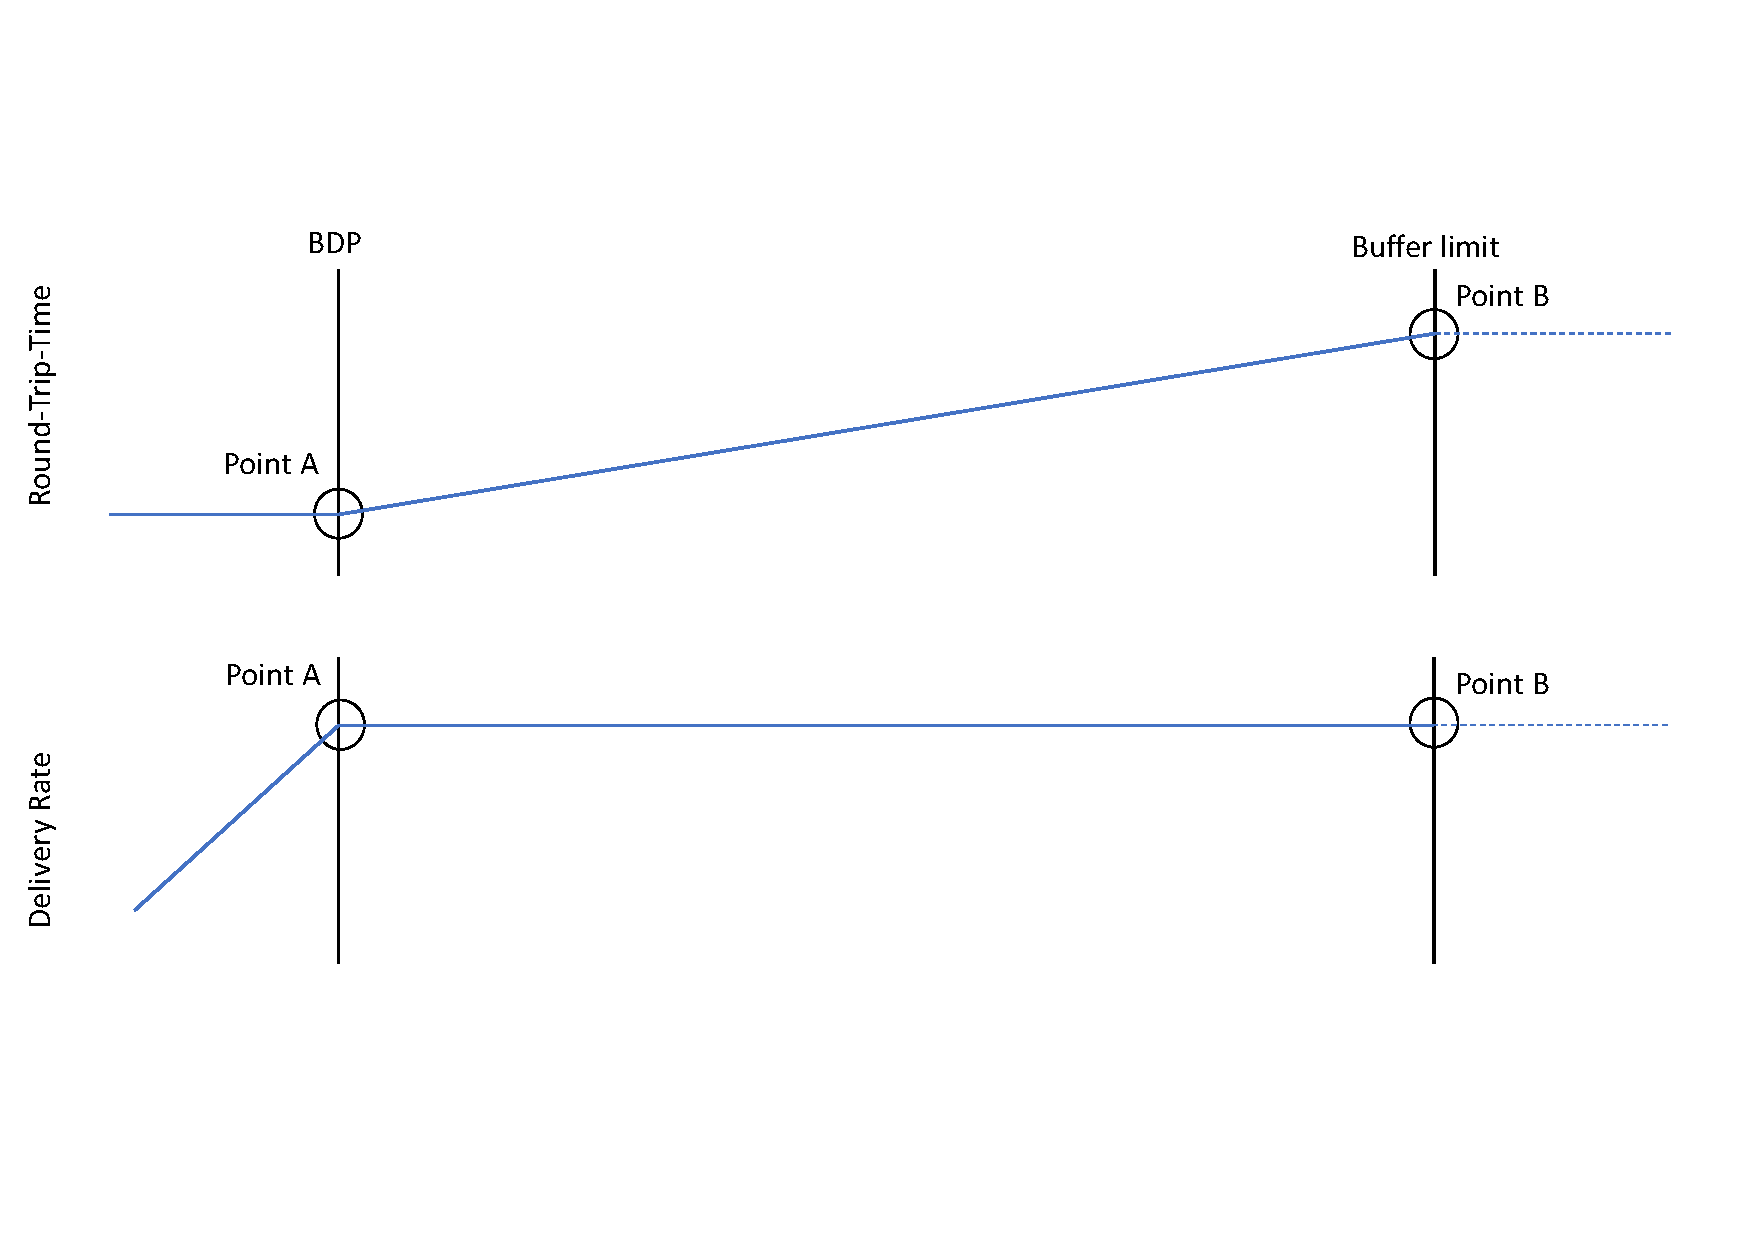
\includegraphics[width=\linewidth]{figures/ProblemForCCAs.pdf}}
\caption{Diagram that shows where different operating points for Congestion COntrol ALgorithms are. Based on \cite{BBRORIGINAL,BBREVALUATION}}
\label{ProblemForCCAS}
\end{figure}

The fundamental goal of a Congestion Control Algorithm is to maximize throughput while maintaining a low delay. 
To determine the ideal performance of such an algorithm, it is necessary to identify the optimal operating point by observing how network dynamics shift as a sender increases its transmission rate. 
As illustrated in \ref{ProblemForCCAS}, the relationship between the sending rate, the delivery rate, and the RTT can be visualized through two primary diagrams. 
The top diagram tracks the RTT, while the bottom diagram displays the delivery rate, highlighting two critical thresholds labeled Point A and Point B.  

Point A represents the moment the delivery rate equals the BDP, indicating that the bottleneck link is fully utilized.
Beyond this point, the delivery rate plateaus because the bottleneck has reached its maximum physical capacity. 
If the sender continues to increase its rate past Point A, the excess packets are forced to accumulate in the bottleneck's buffer, creating a queue. 
This accumulation causes a linear increase in RTT, as seen in the upper diagram of \ref{ProblemForCCAS}, because packets must wait longer in the queue before being processed.  
Eventually, if the rate increases further, the system reaches Point B, which signifies the buffer limit. 
At this stage, the bottleneck can no longer accept new packets, leading to packet drops and severe congestion. 

In addition to these performance metrics, another critical benchmark for evaluating a congestion control algorithm is its fairness toward other flows competing for resources at the bottleneck. 
While the behavior shown in \ref{ProblemForCCAS} suggests that the optimal operating point for an individual sender is exactly at Point A, a high-quality algorithm must also ensure an equitable distribution of bandwidth. 
To quantify this behavior, one of the most widely utilized metrics for measuring the quality of resource distribution is Jain's Fairness Index. 
Therefore, an ideal congestion control algorithm should not only target maximum efficiency but also maintain a harmonious coexistence with concurrent flows to prevent starvation or unfair resource dominance.

\subsection{BBR}

The authors of \cite{BBREVALUATION} conducted an extensive study on the performance and quality of BBR, initially testing it with multiple self-competing flows and subsequently against TCP Cubic flows. 
Their results indicate that multiple concurrent BBR flows tend to overestimate available bandwidth, which leads to persistent queue accumulation at the bottleneck. 
In scenarios involving two BBR flows, for instance, the total BDP can reach twice the actual BDP of the link.  
If the bottleneck possesses a large buffer, it may successfully handle these flows, placing the operating point somewhere between the ideal Point A and the buffer limit at Point B from \ref{ProblemForCCAS}. 
However, if the bottleneck buffer is small, BBR flows operate significantly beyond Point B, resulting in severe packet loss. 
While TCP Cubic also experiences retransmissions in these scenarios, they are significantly less frequent than those observed with BBR. 
Even when the bottleneck buffer size is set to $0.8 \times BDP$, the retransmission rate for BBR remains enormous.

Furthermore, experiments in \cite{BBREVALUATION} demonstrate that BBR faces significant challenges when competing with TCP Cubic flows. 
In large buffers, TCP Cubic tends to fill the queue, making it difficult for BBR to accurately estimate the correct RTT. 
Conversely, in small buffers, BBR suppresses TCP Cubic flows because Cubic interprets the packet loss induced by BBR as a congestion signal and drastically reduces its sending rate. 
Given the high volume of legacy systems still utilizing TCP Cubic, BBR exhibits "unfair" behavior in real-world Internet scenarios

The extensions AQDC BBR and BBR-ES focus on resolving the issue of accumulated packets in the bottleneck queue while offering intrinsic improvements to the core BBR algorithm.
The authors of AQDC BBR demonstrated that their improvements successfully decreased the RTT compared to standard BBR and achieved an 11\% improvement in Jain's Fairness Index. 
This improvement is largely attributed to the algorithm's ability to reduce tail latency by more than 25\% compared to standard BBR, which it achieves by explicitly modeling and compensating for "queue debt" incurred during probing phases. 
By quantifying the excess packets injected during the ProbeBW phase, AQDC BBR prevents the persistent buffer occupancy that typically compromises fairness.

Similar results were produced by the authors of BBR-ES, whose experiments showed that the algorithm maintained lower RTTs than BBR while preserving high link utilization. 
Unlike earlier delay-based variants, BBR-ES utilizes a trend-based transition mechanism and an "Extended State" stabilization phase to manage per-flow bandwidth and RTT evolution. 
These findings were validated in real-world scenarios by sending data to various Amazon EC2 instances in cities such as Tokyo, Singapore, and Virginia across varying throughput levels. 
Their research confirmed that BBR-ES achieves a consistently higher Jain's Fairness Index—often above 0.9—compared to both standard BBR and TCP Cubic. 
Additionally, measurements showed that BBR-ES consistently maintains top-tier link utilization, frequently exceeding 98\% in most experimental settings. 
By monitoring short-term indicators, BBR-ES effectively distinguishes between flows that heavily contribute to queue buildup and those that do not, allowing for targeted corrective actions and overall greater stability.

\subsection{PCC}

To demonstrate that PCC is a stable and effective congestion control algorithm, the authors conducted several comprehensive studies across diverse network environments. 
Their results consistently showed that PCC maintains high throughput and is significantly more resilient to random packet loss than traditional TCP variants. 
For instance, on unreliable lossy links, PCC can maintain over 95\% capacity even at a 1\% loss rate, whereas TCP CUBIC's performance collapses by more than ten times under the same conditions.\cite{PCCEVALUATION} 
This resilience stems from PCC's ability to distinguish between congestive loss and random link errors through its utility-maximizing framework.  

Beyond raw throughput, the studies highlighted PCC's superior reactivity to rapid network changes. 
In experiments where available bandwidth, RTT, and loss rates were modified every five seconds, PCC remained near the optimal sending rate throughout the duration of the test. 
In contrast, alternative algorithms like BBR or TCP CUBIC required significantly more time to converge to the optimum or failed to reach it entirely in such volatile environments. 
Furthermore, PCC proves to be remarkably efficient with limited resources, achieving 90\% throughput with a small buffer size, while TCP CUBIC requires thirteen times more buffer to reach the same level of performance\cite{PCCEVALUATION}. 

A critical component of PCC's evaluation is its behavior when sharing the network with other flows. 
Despite its "selfish" design focused on utility maximization, competing PCC flows are mathematically and empirically shown to converge to a stable and fair equilibrium. 
This includes strong RTT fairness, where flows with different propagation delays receive their fair share of bandwidth rather than the shorter-RTT flow dominating the link—a common flaw in protocols like TCP CUBIC. 
Regarding TCP friendliness, while "classic" PCC is designed to outperform legacy congestion control algorithms, the framework can be adjusted to be more "socially" compatible with traditional flows, ensuring that PCC does not completely starve existing flows traffic in mixed-protocol environments.

\subsection{Copa}

\subsubsection{Basic Copa}

The primary objective of the Copa authors was to develop a congestion control algorithm that is both high-performing and simple to understand. 
While evaluating an algorithm's "simplicity" is inherently subjective and less straightforward than quantitative metrics, several comparisons highlight Copa's relatively low complexity.  

For instance, PCC is built upon a framework that uses online learning and utility maximization, which can be complex to reason about due to its continuous "micro-experiments" of different sending rates. 
In contrast, Copa's core design centers on a single target rate equation: $\lambda = 1/(\delta d_q)$, where $d_q$ represents the measured queuing delay. 
While the derivation of this formula involves advanced modeling, the resulting algorithm remains highly comprehensible.  

Furthermore, Copa operates in two distinct modes to ensure versatility: a default mode for low-latency performance and a competitive mode designed to match the aggressiveness of buffer-filling schemes like TCP Cubic. 
The transition between these modes is determined by straightforward measurements.
The sender switches to competitive mode if it fails to detect a "nearly empty" queue within a 5-RTT window. 
While BBR also relies on limited parameters — specifically its estimates of Bottleneck's Bandwidth and RTT — PCC adopts a more data-intensive approach, continuously aggregating various packet-level events (such as loss, throughput, and latency) into a utility function to determine its sending rate.

Overall, Copa is not the most difficult algorithm to understand, particularly when compared to other modern schemes. 
We have determined that, in contrast to algorithms like PCC—which utilizes complex online optimization and randomized controlled trials—Copa relies on a more transparent, delay-based target rate formula. 
While PCC's decision-making involves aggregating multiple packet-level events into a performance utility function, Copa's logic is driven by a straightforward relationship between sending rate and queuing delay. 
Therefore, we conclude that the authors successfully reached their goal of creating a high-performing congestion control algorithm that remains simple for humans to reason about.

We will now examine the performance of Copa. 
The authors evaluated the algorithm through various experiments, comparing it directly with other prominent congestion control schemes, including PCC, BBR, and TCP Cubic. 
A central component of this evaluation is Copa's core mechanism: the target rate equation, $\lambda = 1/(\delta d_q)$.  
In one specific set of results, the authors presented Copa's performance with the competitive mode disabled. 
These findings demonstrate that in its default mode, Copa is exceptionally effective, achieving near-ideal values for both throughput and RTT estimation. 
Specifically, when operating in this mode, Copa stabilizes at a point that optimizes the trade-off between throughput and delay, effectively reaching the optimal "Point A" described in \ref{ProblemForCCAS}. 
However, the authors noted that while enabling the competitive mode allows Copa to coexist with buffer-filling flows, this transition results in significantly higher queuing delays and a deviation from these ideal performance metrics.

Furthermore, the authors conducted experiments to evaluate how their algorithm manages a varying number of flows by adding and terminating flows within an emulated network. 
They did the same for BBR, PCC and TCP Cubic.
The results indicate that Copa and TCP Cubic are most effective at maintaining ideal throughput and achieving a high Jain's fairness index, with Copa reaching a median index of 0.86 compared to TCP Cubic's 0.81. 
In contrast, BBR and PCC showed lower median fairness indices of 0.61 and 0.35, respectively. 
Moreover, the study demonstrates that Copa significantly outperforms PCC and BBR in handling changing network conditions, as it converges quickly to correct fair rates.

\subsubsection{Upgrades of Copa (Copa+ and Copa-D)}

Although Copa demonstrates strong performance, the authors of Copa+ and Copa-D identified a significant limitation: the algorithm frequently triggers its competitive mode unnecessarily. 
This premature switching leads to unintended queue accumulation at the bottleneck, compromising the low-latency benefits of its default state. 
Consequently, while Copa achieves near-optimal performance in isolation, the activation of its competitive mode often degrades its overall efficiency, even in isolation. 
To address this, extensions such as Copa+ and Copa-D introduce refined mechanisms for mode-switching logic. 
Specifically, Copa+ incorporates an additional control parameter, while Copa-D utilizes a redefined expression for $\delta$.

Copa+ utilizes this supplemental parameter to prevent erroneous transitions into competitive mode, a claim supported by the authors' experimental results. 
The algorithm consistently maintains RTT values that align with the ideal targets, effectively mirroring the performance of standard Copa when its competitive mode is disabled. 
Therefore, Copa+ successfully addresses the primary flaw of unnecessary mode switching. 
However, as the authors do not provide specific throughput statistics, a definitive conclusion regarding its impact on link utilization cannot be reached.

The authors of Copa-D evaluated their algorithm through several experiments, including scenarios where the available bandwidth was varied at fixed intervals. 
By comparing Copa with their proposed upgrade, Copa-D, they demonstrated how bandwidth fluctuations influence RTT. 
While standard Copa exhibited a highly volatile RTT, Copa-D remained relatively stable. 
This stability is expected since the experiment does not introduced delay, which therefore should ideally not trigger an RTT increase.
However, standard Copa's RTT rose with some bandwidth changes, probably due to unnecessary mode switching while Copa-D maintained a lower average RTT than the original algorithm.

It is noteworthy, however, that the experimental results indicate that Copa-D's RTT oscillates around a target value. 
Interestingly, when standard Copa stabilizes at that same point, its oscillations appear smaller than those of Copa-D. 
The authors attribute this behavior of Copa-D to the dynamic adjustment of $\delta$, which, while stabilizing the average RTT, introduces more frequent minor fluctuations.

Furthermore, the authors tested Copa-D in 4G and 5G network environments. 
Their findings reveal that while standard Copa achieves a slightly higher throughput, its RTT is significantly higher than that of Copa-D. 
This indicates that Copa-D successfully prioritizes lower delay, providing a more stable performance profile in mobile network scenarios.

In summary, Copa represents a compelling congestion control algorithm due to its inherent simplicity and robust performance. 
Through extensions such as Copa+ and Copa-D, the protocol can be tailored to operate efficiently across various specialized use cases. 
However, a significant gap remains regarding its performance in real-world network environments. 
Existing studies primarily rely on controlled experiments, leaving it unclear how effectively Copa and its variants perform outside of emulated settings.
On the public internet, flows rarely exist in isolation.
Instead, multiple heterogeneous algorithms compete for the same bottleneck resources. 
Notably, the evaluations for Copa+ and Copa-D do not adequately address scenarios where the competitive mode is essential, such as when sharing a link with aggressive, buffer-filling protocols like TCP Cubic. 
Consequently, further research is required to determine if these refinements maintain their advantages when faced with the diverse and unpredictable traffic patterns of the global internet.

\subsection{PowerTCP}

The authors of PowerTCP designed their congestion control algorithm specifically for data center networks rather than the public internet. 
This targeted approach is significant because it allows the algorithm to leverage the unique characteristics of controlled environments. 
Unlike the broader internet, a data center is typically managed by a single entity that can mandate the use of specific protocols across the entire infrastructure. 
Consequently, the authors' use of a fat-tree topology for their test environment closely reflects real-world data center network conditions. 
Furthermore, this controlled setting eliminates the need to accommodate legacy systems or outdated congestion control algorithms, which are rarely a factor in modern data center deployments.

The experimental results demonstrate that PowerTCP reacts rapidly and accurately to congestion while maintaining high throughput. 
A key performance indicator is the algorithm's ability to maintain a near-empty queue at the bottleneck, suggesting that PowerTCP operates close to the ideal operating point A described in \ref{ProblemForCCAS}. 
When additional flows are introduced, the algorithm ensures a fair distribution of bandwidth. 
Although the authors do not utilize standard fairness measures like Jain's Fairness Index for direct comparison, independent research \cite{TCPSTHIRDEYE} has successfully reproduced these findings. 
These independent studies confirm that while TCP Cubic consistently fills buffers—resulting in increased queuing delay—PowerTCP maintains minimal occupancy. 
Additionally, PowerTCP flows remain stable and equitable when sharing a bottleneck, whereas TCP Cubic flows often exhibit instability or unfair dominance.

A critical aspect of the authors' evaluation was the impact of PowerTCP on different flow durations, categorized as short, medium, and long flows. 
Their data proves that short flows receive the most significant performance benefits, while medium flows show moderate improvements. 
Long flows also perform effectively, showing no degradation in performance when compared to traditional algorithms. 
This overall efficiency is primarily driven by INT, which provides PowerTCP with a comprehensive real-time view of the network status.

In summary, PowerTCP is highly effective within its specialized niche. 
It successfully achieves high throughput with minimal delay by preventing queue buildup. 
However, its heavy reliance on INT represents a significant limitation.
It is highly improbable that routers or switches in the wide-area internet would provide the necessary telemetry data that the algorithm requires. 
Therefore, while PowerTCP is an optimal choice for congestion control within a data center, it lacks a viable use case in general networking environments where telemetry requirements cannot be met.

\subsection{C4}

The authors of the C4 algorithm primarily focused on optimizing network flows for real-time media, such as video and audio streams, which are highly sensitive to latency and queuing delays. 
In their findings published in the C4 repository, the algorithm was rigorously compared against BBR and TCP Cubic within various simulated WiFi network environments. 
These evaluations encompassed scenarios such as WiFi suspension, fading, and extreme jitter to determine C4's robustness relative to its peers. 
In high-bandwidth basic tests, C4 and Cubic performed identically with minimal delay, whereas BBR's pacing logic resulted in a maximum audio queuing delay of significant higher than the delay observed for C4. 
Under low-bandwidth conditions (10 Mbps), C4 demonstrated a superior ability to manage high-definition video, maintaining a maximum delay than that from BBR. 
Furthermore, during extreme jitter tests, C4 utilized tighter transmission control by pacing traffic at approximately 29 Mbps for a 20 Mbps link while BBR is pacing at 58 Mbps, which successfully prevented video spikes from interfering with high-priority audio traffic. 
Even in challenging suspension scenarios, C4 proved to be more efficient than TCP Cubic and neared the performance levels of BBR, illustrating its effectiveness as a modern congestion control solution for media-heavy applications.

In summary, current evaluations of C4 are limited by a lack of performance data regarding its behavior in network environments beyond Wi-Fi. 
Furthermore, there is an absence of empirical evidence concerning its fairness when competing with other flows or just multiple flows of its own, as the provided datasets do not address how C4 interacts with diverse traffic types. 
Given its demonstrated advantages over TCP Cubic and BBR in wireless scenarios—particularly in reducing queuing delay for real-time media—C4 warrants further testing in varied network architectures to determine if its effectiveness persists across different environments. 
Additionally, a significant research gap exists because there is no direct comparison between C4 and the Copa algorithm or its extensions. 
While existing data suggests that Copa might offer competitive performance, a definitive conclusion cannot be reached because the respective tests were conducted in disparate network conditions, making a direct side-by-side evaluation impossible at this time.



\section{Summary}\label{sec:Summary}

Congestion control has been an active area of research for over 40 years, evolving rapidly in response to the massive increase in global network traffic. 
The first mentioned \ac{CCA} is BBR which was developed by Google and aimed at using a different technique to control a flow than older \ac{CCA}s do.
Althought the approach is already good, it is not perfect which led to the developement of BBR-ES and AQDC BBR which are extensions and upgrades to BBR and they target the weaknesses of BBR.
As the further need for effective congestion control grew, the complexity of these algorithms increased significantly. 
A prime example of this complexity is PCC, which replaces traditional hard-wired logic with a data-intensive framework of online learning, "micro-experiments," and utility maximization.  

This trend toward sophistication has sparked a "counter-movement" aimed at making algorithms, such as Copa, more transparent and easier for humans to reason about. 
Although Copa is already very good, it has some problems which is mainly, that it switches sometimes into its competetive mode, although it is not necessary.
To solve this there are newer versions of Copa developed which are Copa+ and Copa-D.
Both tackle the problem of Copa in there own way very good.
Another new approach for a \ac{CCA} is C4 which is bringing a new concept to the table that has similarities to BBR.
Due to its recent emergence, peer-reviewed sources and data are currently limited.

Modern development is now defined by high specialization. 
Algorithms like Copa-D are tailored for the volatility of mobile networks, while PowerTCP is optimized for data centers by leveraging INT.  
However, this specialization makes comparative analysis difficult, as an algorithm's behavior changes across different network types. 
Furthermore, because most performance data is derived from tests in controlled, specialized environments, it remains a challenge to benchmark these algorithms against one another or predict their effectiveness in the diverse conditions of the global internet.
Despite this lack of common ground in testing environments, Jain's Fairness Index serves as a vital, relatively consistent metric for the field. 


\section{Outlook}\label{sec:Outlook}

The future of congestion control is not yet written, as a "perfect" universal algorithm has yet to be realized. 
Consequently, there will remain a significant research focus on the field to ensure that algorithms can consistently maintain the optimal operating point, identified as Point A in \ref{ProblemForCCAS}, where the bottleneck link is fully utilized without creating a queue. 
Future developments will likely become increasingly specialized for distinct environments, such as the unique demands of datacenter networks, the volatility of 4G and 5G mobile networks, or the broad unpredictability of the general internet. 
Furthermore, with the continued increase in satellite communication, this area will become even more critical to the evolution of congestion control. 
While emerging research is already addressing the specific challenges of satellite links, those studies remained outside the scope of this paper. 
Ultimately, the next generation of algorithms must reconcile the need for high performance with the necessity for architectural simplicity and fairness in a multi-protocol world.




\bibliographystyle{IEEEtran}
\bibliography{seminar-paper}

\end{document}
